\documentclass{article}
\usepackage{kantlipsum,xgalley,tikz}
\ExplSyntaxOn
\box_new:N \l_xwrapfig_fig_box
\box_new:N \l_xwrapfig_vfig_box
\box_new:N \l_xwrapfig_hfig_box
\dim_new:N \l_xwrapfig_wd_dim
\dim_new:N \l_xwrapfig_totalht_dim
\dim_new:N \l_xwrapfig_adjwd_dim
\clist_new:N \l_xwrapfig_indents_clist
\int_new:N \l_xwrapfig_lines_int
\int_new:N \l_xwrapfig_totallines_int
\int_new:N \l_xwrapfig_adjlines_int
\fp_new:N \l_xwrapfig_adjfig_fp
\dim_set:Nn \l_xwrapfig_adjwd_dim { 2ex }
\int_set:Nn \l_xwrapfig_adjlines_int { 1 }
\cs_generate_variant:Nn \galley_cutout_right:nn { nV }
\cs_generate_variant:Nn \galley_cutout_left:nn { nV }
\cs_new_protected:Nn \xwrapfig_prewrap:n
{
  \clist_clear:N \l_xwrapfig_indents_clist
  \vbox_set:Nn \l_xwrapfig_vfig_box { #1 }
  \dim_set:Nn \l_xwrapfig_totalht_dim { \box_ht:N \l_xwrapfig_vfig_box + \box_dp:N \l_xwrapfig_vfig_box }
  \hbox_set:Nn \l_xwrapfig_hfig_box { #1 }
  \dim_set:Nn \l_xwrapfig_wd_dim { \box_wd:N \l_xwrapfig_hfig_box + \l_xwrapfig_adjwd_dim }
  \int_set:Nn \l_xwrapfig_totallines_int { ( \l_xwrapfig_totalht_dim / \baselineskip ) + \l_xwrapfig_adjlines_int }
  \int_zero:N \l_xwrapfig_lines_int
  \int_do_while:nn { \l_xwrapfig_lines_int < \l_xwrapfig_totallines_int }
  {
    \int_incr:N \l_xwrapfig_lines_int
    \clist_put_right:Nn \l_xwrapfig_indents_clist { \l_xwrapfig_wd_dim }
  }
}
\cs_new_protected:Nn \xwrapfig_postwrap:
{
  \box_set_ht:Nn \l_xwrapfig_fig_box { 0pt }
  \box_set_dp:Nn \l_xwrapfig_fig_box { 0pt }
  \box_use:N \l_xwrapfig_fig_box
}
\cs_new_protected:Nn \xwrapfig_putright:nn
{
  \xwrapfig_prewrap:n { #2 }
  \galley_cutout_right:nV { #1 } \l_xwrapfig_indents_clist
  \vbox_set:Nn \l_xwrapfig_fig_box
  {
    \fp_set:Nn \l_xwrapfig_adjfig_fp { ( #1 + .5\l_xwrapfig_adjlines_int ) * \baselineskip }
    \skip_vertical:n  { \fp_to_dim:N \l_xwrapfig_adjfig_fp }
    \hbox_to_wd:nn { \linewidth } { \skip_horizontal:n { \linewidth - \l_xwrapfig_wd_dim + .5\l_xwrapfig_adjwd_dim } #2 }
  }
  \xwrapfig_postwrap:
}
\cs_new_protected:Nn \xwrapfig_putleft:nn
{
  \xwrapfig_prewrap:n { #2 }
  \galley_cutout_left:nV { #1 } \l_xwrapfig_indents_clist
  \vbox_set:Nn \l_xwrapfig_fig_box
  {
    \fp_set:Nn \l_xwrapfig_adjfig_fp { ( #1 + .5\l_xwrapfig_adjlines_int ) * \baselineskip }
    \skip_vertical:n  { \fp_to_dim:N \l_xwrapfig_adjfig_fp }
    \hbox_to_wd:nn { \l_xwrapfig_wd_dim } { \skip_horizontal:n { .5\l_xwrapfig_adjwd_dim } #2 }
  }
  \xwrapfig_postwrap:
}
\NewDocumentCommand\putright { O { 2 } +m }
{
  \xwrapfig_putright:nn { #1 } { #2 }
}
\NewDocumentCommand\putleft { O { 2 } +m }
{
  \xwrapfig_putleft:nn { #1 } { #2 }
}
\ExplSyntaxOff

\begin{document}

\putright[0]{%
  \begin{tikzpicture}
    \newcommand*\len{1.5}
    \draw [thick] (0,0,\len) coordinate (a) \foreach \i/\j in {(\len,0,\len)/b,(\len,0,0)/c,(\len,\len,0)/g,(0,\len,0)/h,(0,\len,\len)/e,(\len,\len,\len)/f} {-- \i coordinate (\j)} -- (g) (f) -- (b) (a) -- (e);
    \coordinate (d) at (0,0,0);
    \draw [gray] (a) -- (d) edge (c) -- (h);
    \foreach \i/\j in {a/left,b/right,c/right,d/left,e/left,f/right,g/above,h/above} \node at (\i) [\j] {\i};
  \end{tikzpicture}}
Let $G S_8$ and $X = \{\{a,g\},\{b,h\},\{c,e\},\{d,f\}\}$\par
\kant[1-2]

\putleft[3]{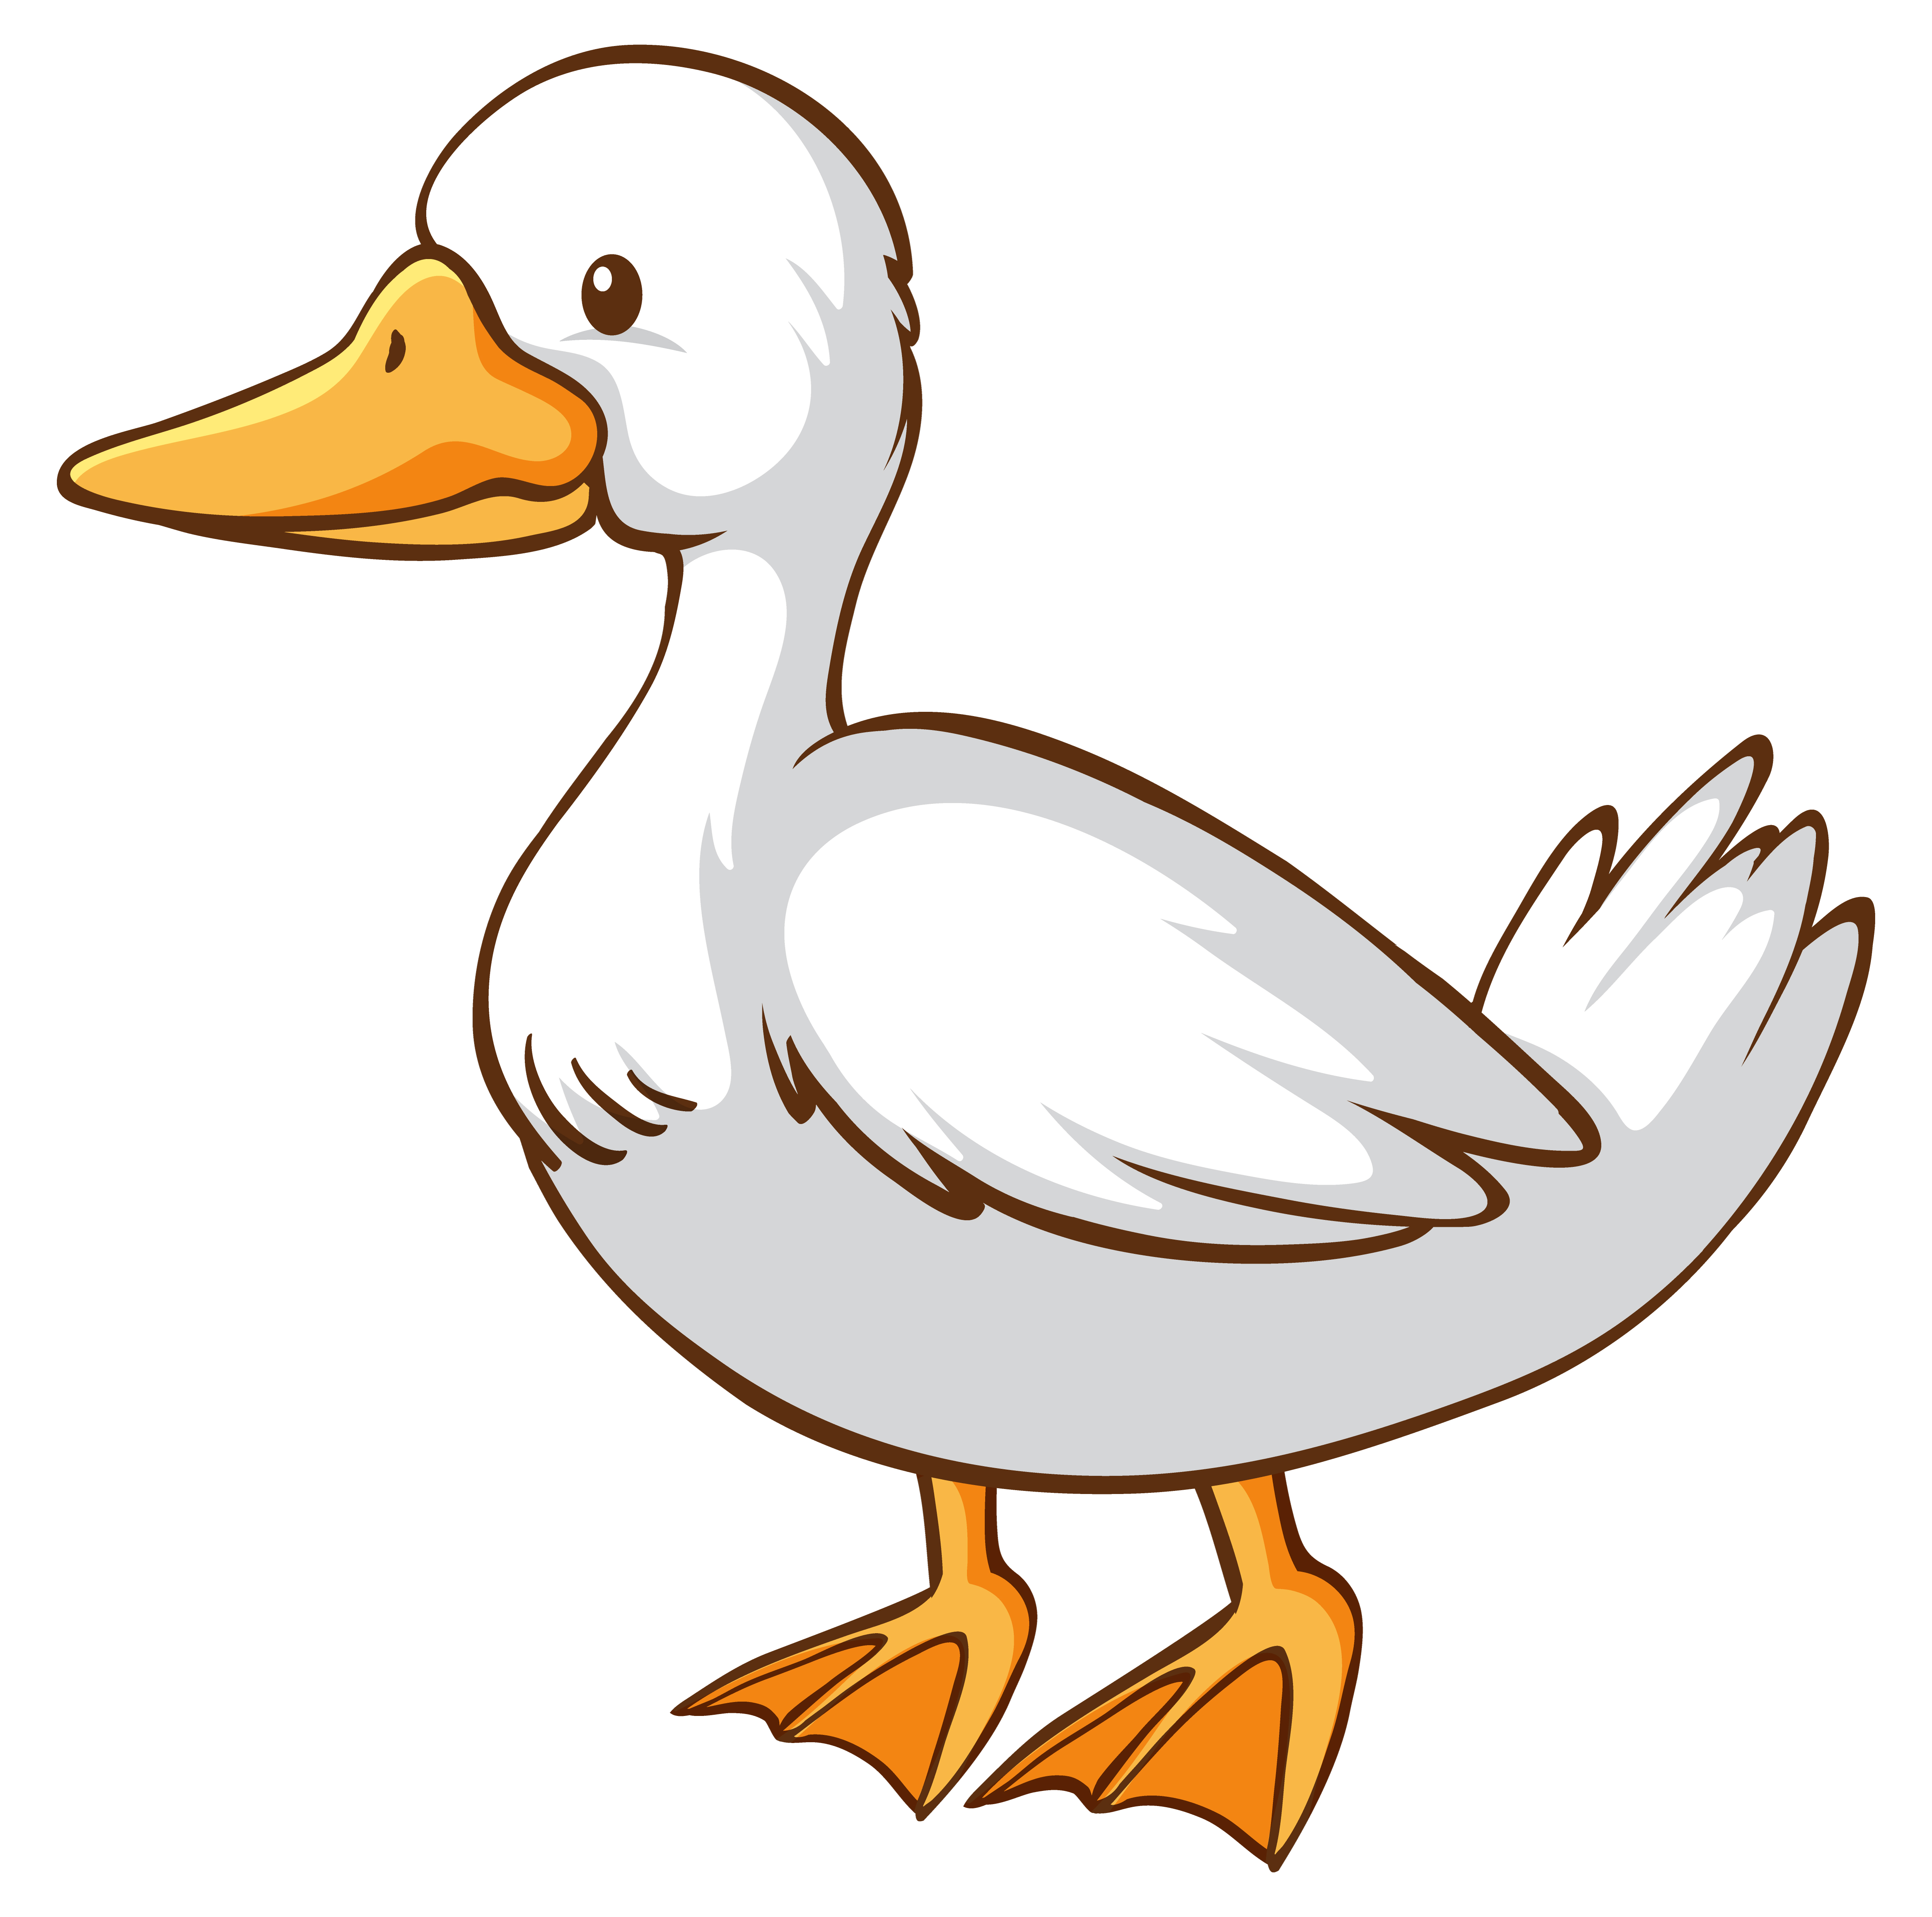
\includegraphics[width=.3\textwidth]{duck}}
\kant[3]
\clearpage

\putleft[0]{%
  \begin{tikzpicture}
    \newcommand*\len{1.5}
    \draw [thick] (0,0,\len) coordinate (a) \foreach \i/\j in {(\len,0,\len)/b,(\len,0,0)/c,(\len,\len,0)/g,(0,\len,0)/h,(0,\len,\len)/e,(\len,\len,\len)/f} {-- \i coordinate (\j)} -- (g) (f) -- (b) (a) -- (e);
    \coordinate (d) at (0,0,0);
    \draw [gray] (a) -- (d) edge (c) -- (h);
    \foreach \i/\j in {a/left,b/right,c/right,d/left,e/left,f/right,g/above,h/above} \node at (\i) [\j] {\i};
  \end{tikzpicture}}
Let $G S_8$ and $X = \{\{a,g\},\{b,h\},\{c,e\},\{d,f\}\}$\par
\kant[4]

\putright{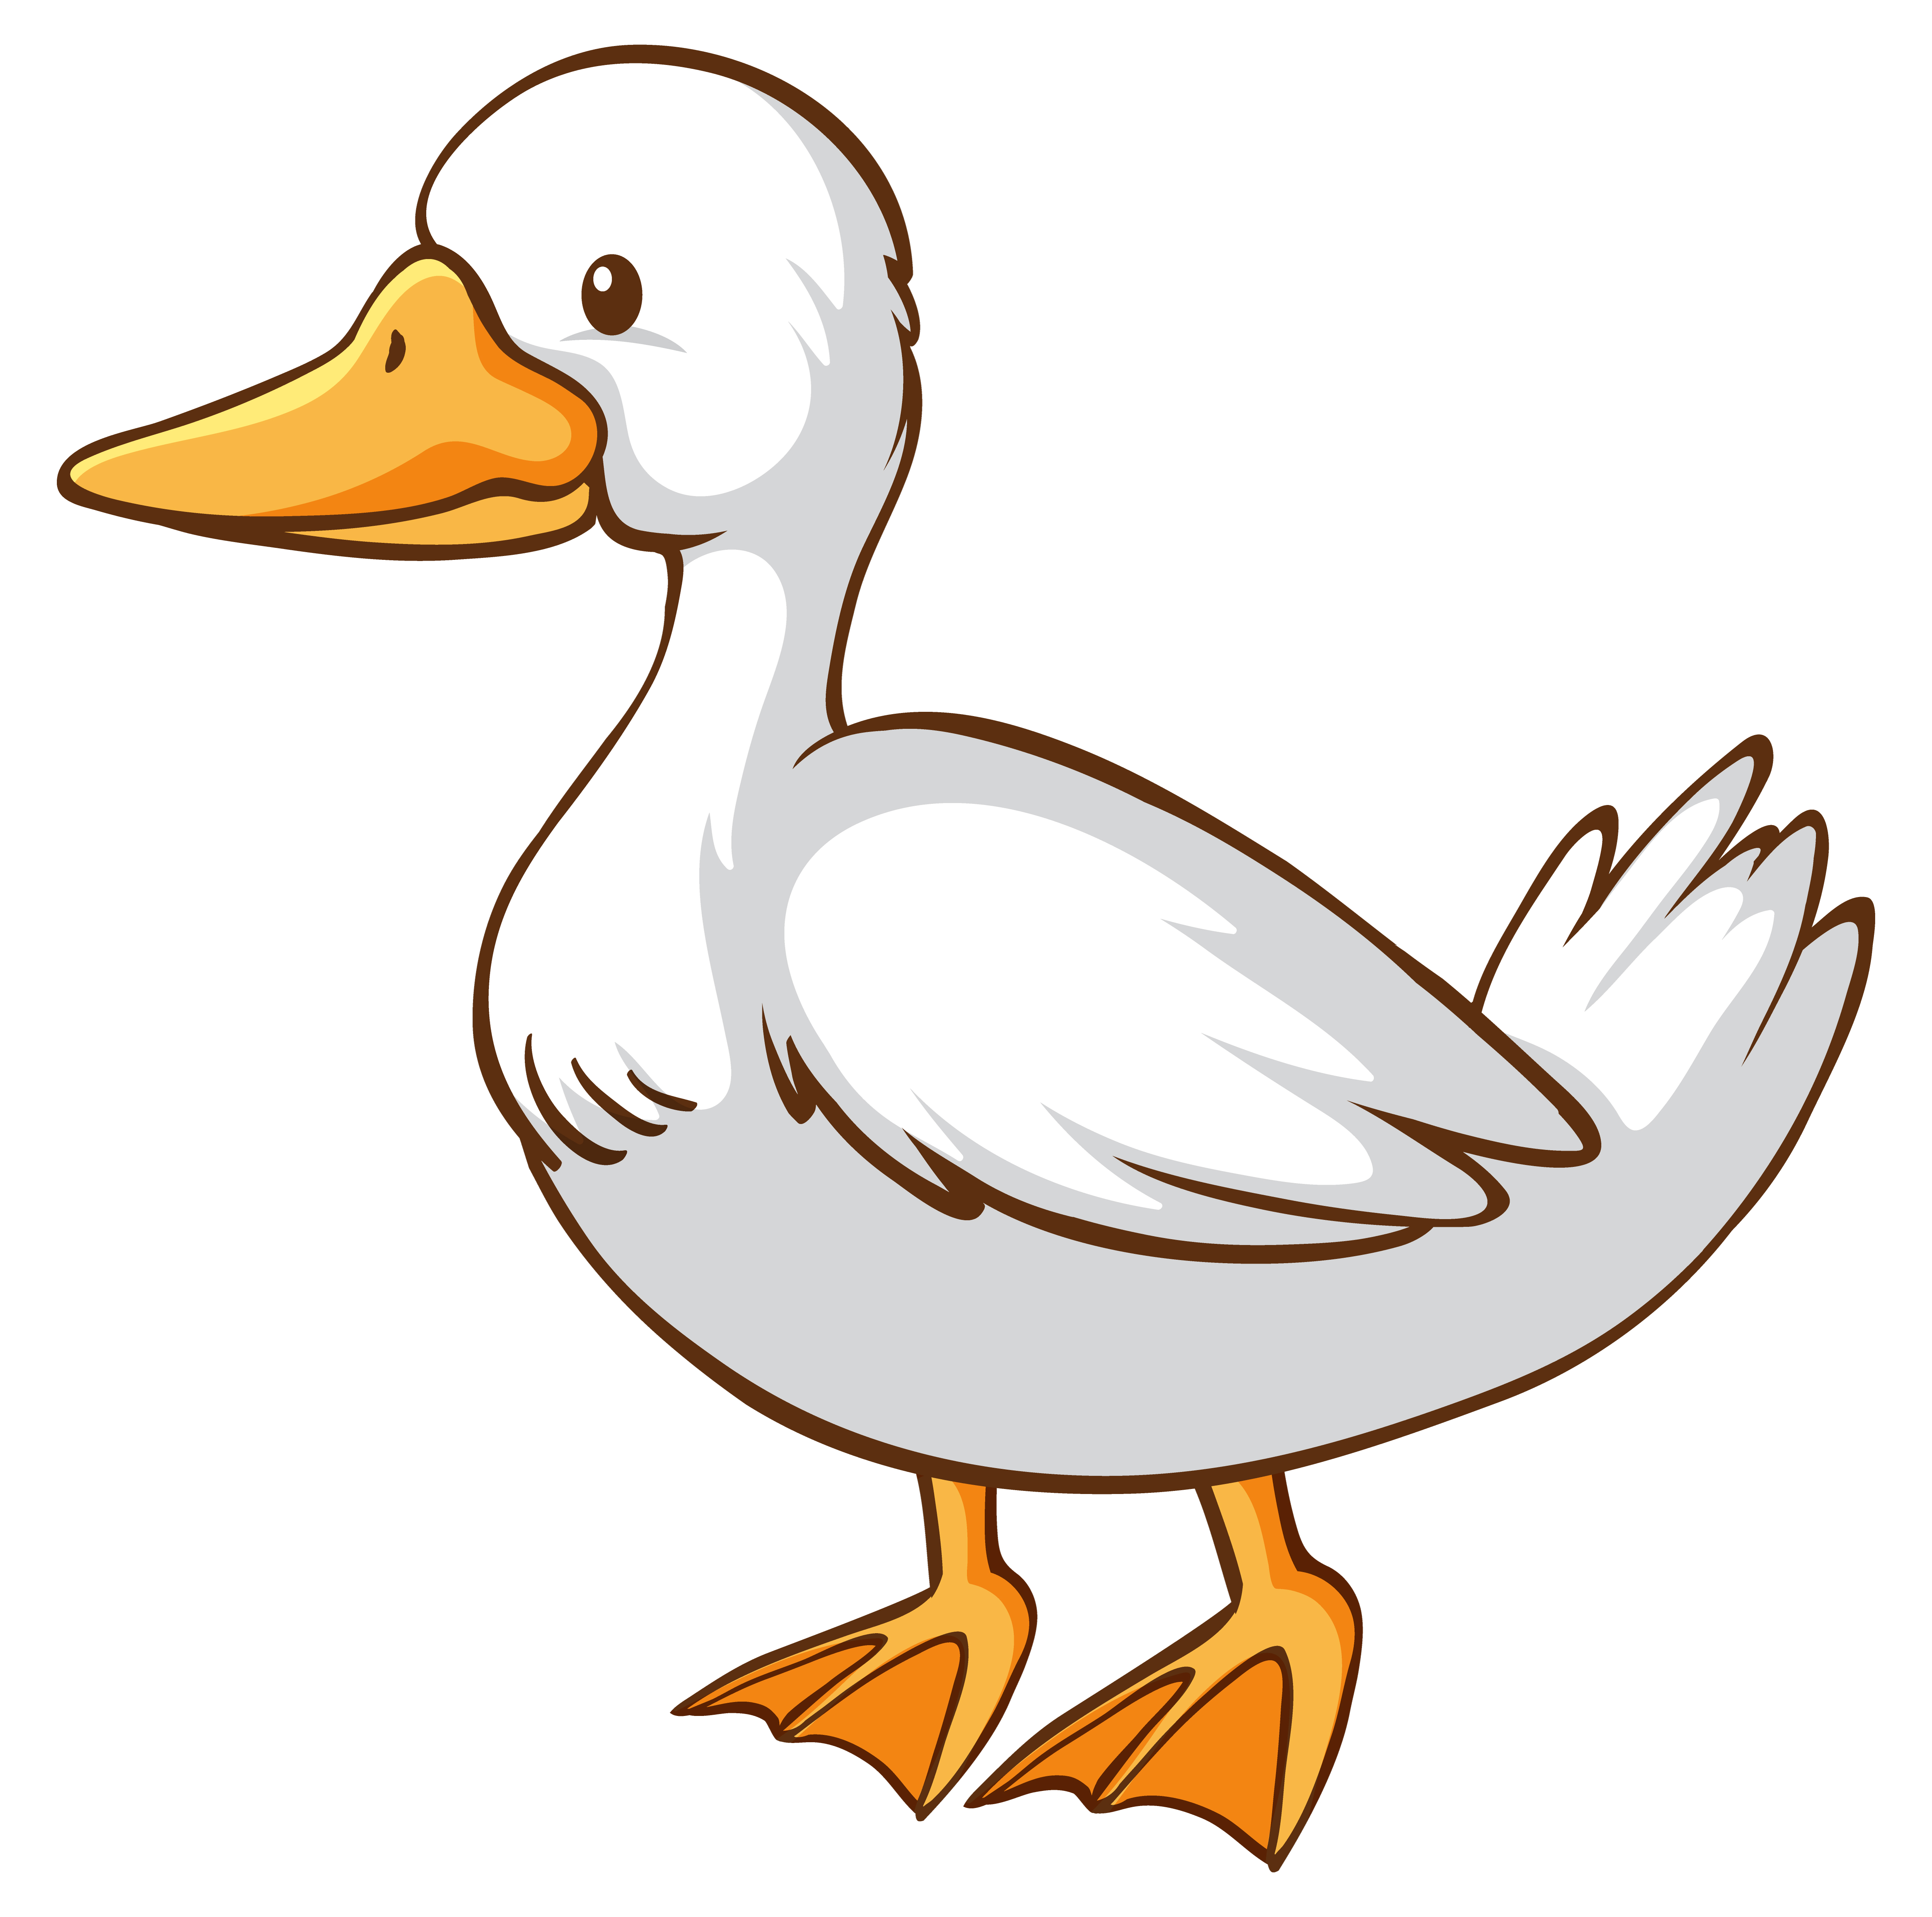
\includegraphics[width=.3\textwidth]{duck}}
\kant[5]

\end{document}